\providecommand{\main}{../../..}
\documentclass[\main/main.tex]{subfiles}
\begin{document}

\subsection{Esercizio 3}
Si descriva brevemente il metodo dei vincoli per enumerare le soluzioni paretiane, specificandone vantaggi e svantaggi.

Si applichi tale metodo al problema seguente risolvendo graficamente i sottoproblemi richiesti.

\begin{align*}
  \min f_1(x) & = x_1^2 + x_2^2 + x_1                            \\
  \min f_2(x) & = -x_1                                           \\
  X           & = \{x:x_1 \geq 0, x_2 \geq 0, x_1 + x_2 \leq 2\}
\end{align*}

\subsection{Soluzione esercizio 3}
\subsubsection*{Il metodo dei vincoli}
Il teorema su cui si basa questo metodo afferma che un punto di ottimo globale $x^o$ per gli indicatori $f_l$ è punto di ottimo globale anche per il problema costruito come:

\begin{align*}
  \min f_{l^*}(x)                                                                      \\
  f_l(x) & \leq \epsilon_l = f_l(x^o) \qquad l \in \{1,\ldots,p\}  \setminus \{ l^* \}
\end{align*}

Si procede vincolando al valore ottimo assunto dall'indicatore $\epsilon_l = f_l(x^o)$ l'indicatore $l-esimo$ e quindi si può identificare il valore dello standard $\epsilon_l$ e quindi $x^o$ risolvere tramite KKT o graficamente.

\subsubsection*{Vantaggi}
\begin{enumerate}
  \item È sempre applicabile.
\end{enumerate}

\subsubsection*{Svantaggi}
\begin{enumerate}
  \item Produce una sovrastima di $X^o$.
  \item In problemi con molti indicatori l'identificazione dei vari standard può risultare ardua.
\end{enumerate}

\subsubsection*{Risoluzione con metodo dei vincoli}
Riformulo il problema:
\begin{align*}
  \min f_1(x) & = x_1^2 + x_2^2 + x_1 \\
  x_1         & \geq 0                \\
  x_2         & \geq 0                \\
  x_1 + x_2   & \leq 2                \\
  -x_1        & \leq \epsilon_2
\end{align*}

È chiaro che la funzione $f_1$ sia un cerchio con centro in $C = (-\frac{1}{2}, 0)$, che quindi coincide con il punto di minimo globale non vincolato. In base ai vincoli che costringono la $x_1$, lo standard $\epsilon_2 \in [-2, \infty)$, ma oltre $\epsilon_2 \in [-2, 0]$ i valori perdono di interesse per il problema.

\begin{figure}
  \begin{subfigure}{0.45\textwidth}
    \begin{tikzpicture}
      \begin{axis}[


          xlabel=$x_1$,
          ylabel=$x_2$,
          zlabel=$f(x)$
        ]
        \addplot3[surf, unbounded coords=jump]
        {x > 0 && y>0 && x+y<2 ? y^2 + x^2 +x : NaN};
      \end{axis}
    \end{tikzpicture}
    \caption{La funzione $f_1(x)$ nel suo dominio}
  \end{subfigure}
  ~
  \begin{subfigure}{0.45\textwidth}
    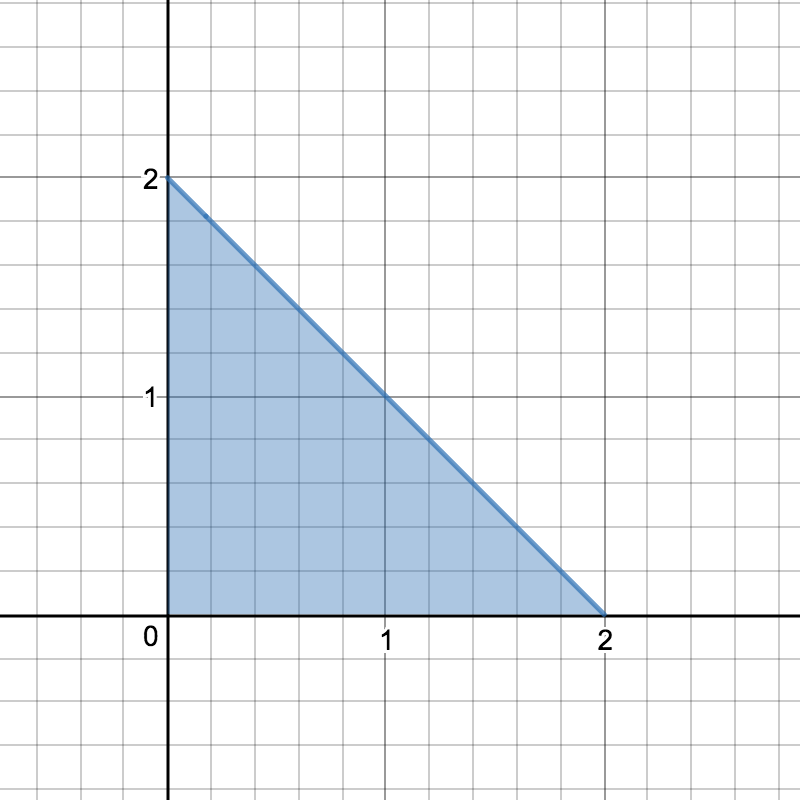
\includegraphics[width=0.8\textwidth]{es3-20160302}
    \caption{Dominio delle soluzioni}
  \end{subfigure}
\end{figure}

\begin{figure}
  \begin{subfigure}{0.32\textwidth}
    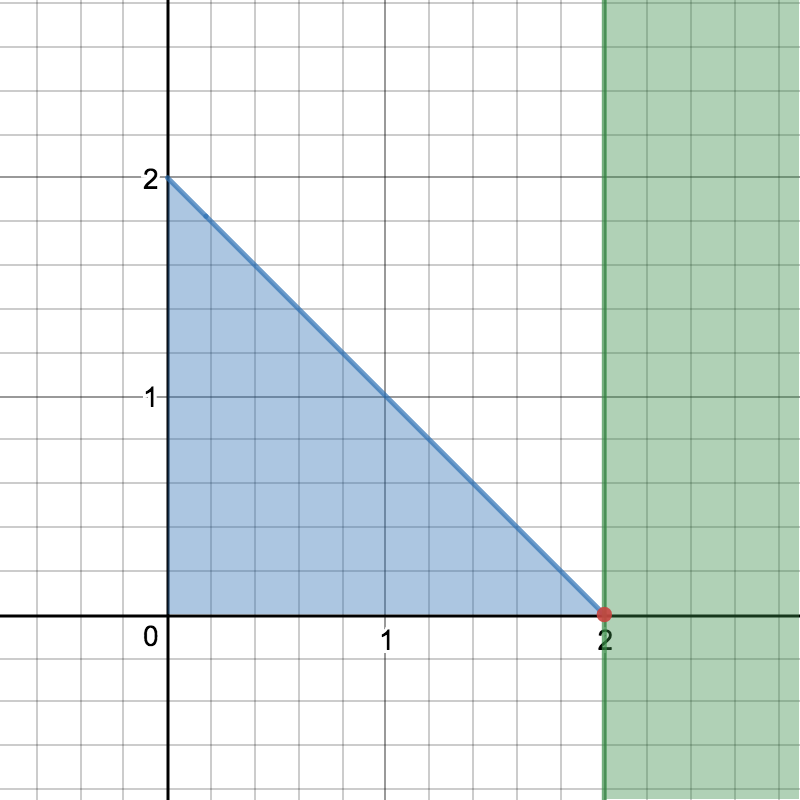
\includegraphics[width=\textwidth]{es3-20160302-1}
    \caption{Caso $\epsilon_2 \geq -2$ l'unico ottimo globale è $A = (2,0)$.}
  \end{subfigure}
  ~
  \begin{subfigure}{0.32\textwidth}
    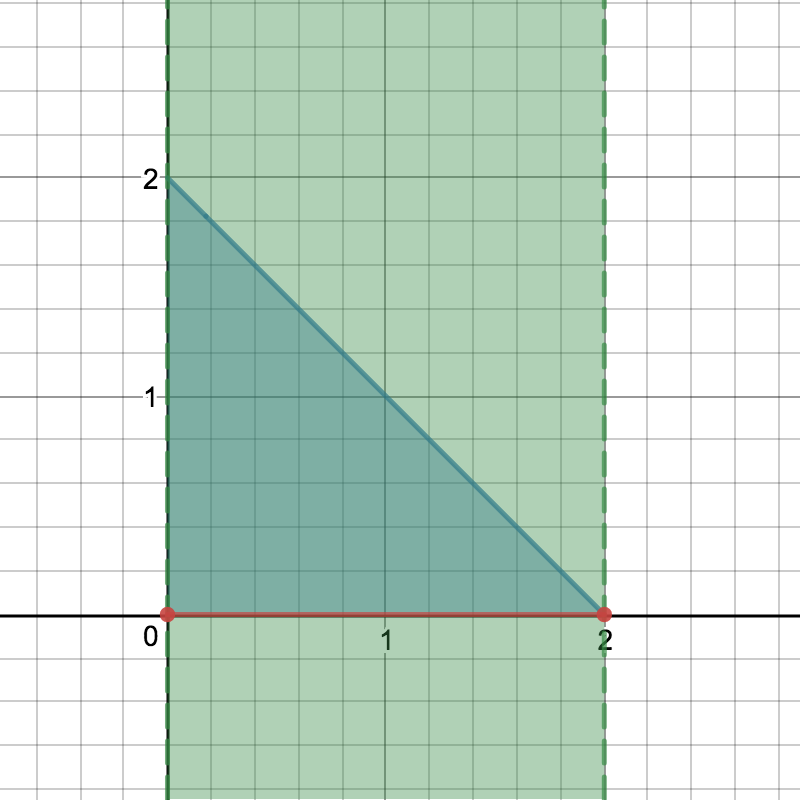
\includegraphics[width=\textwidth]{es3-20160302-2}
    \caption{Caso $-2<\epsilon_2 \leq 0$, l'ottimo si sposta gradualmente da $A$ a $B = (0,0)$.}
  \end{subfigure}
  ~
  \begin{subfigure}{0.32\textwidth}
    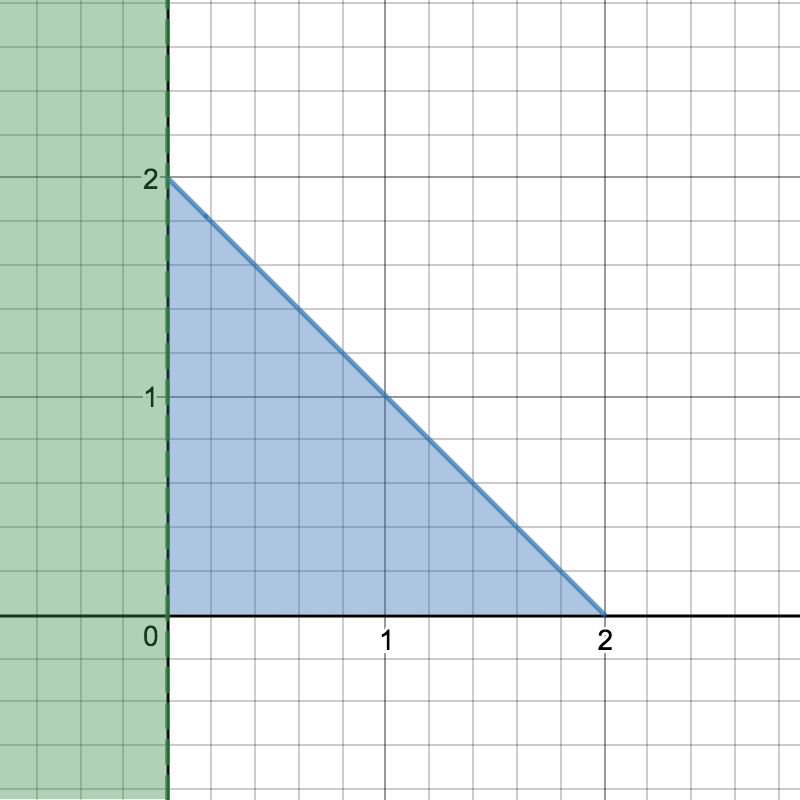
\includegraphics[width=\textwidth]{es3-20160302-3}
    \caption{Nel caso $\epsilon_2 > 0$ non vi sono più soluzioni nel dominio di definizione.}
  \end{subfigure}
\end{figure}

La regione paretiana quindi è il segmento tra il punto $A$ e $B$.

\end{document}